% Chapter 1

\chapter{Introducción general} % Main chapter title

\label{Chapter1} % For referencing the chapter elsewhere, use \ref{Chapter1} 
\label{IntroGeneral}

En el presente capítulo se presentan los diferentes métodos de control de acceso en el ámbito de Internet de las Cosas y se expone la motivación que impulsa este trabajo, los objetivos y el alcance definidos.

%----------------------------------------------------------------------------------------

% Define some commands to keep the formatting separated from the content 
\newcommand{\keyword}[1]{\textbf{#1}}
\newcommand{\tabhead}[1]{\textbf{#1}}
\newcommand{\code}[1]{\texttt{#1}}
\newcommand{\file}[1]{\texttt{\bfseries#1}}
\newcommand{\option}[1]{\texttt{\itshape#1}}
\newcommand{\grados}{$^{\circ}$}

%----------------------------------------------------------------------------------------

%\section{Introducción}

%----------------------------------------------------------------------------------------
\section{Estado del arte}

Es esta sección se presenta una introducción a las soluciones IoT y su uso para gestionar el control de acceso en las empresas.

\subsection{Tecnología IoT}

Con la expansión de Internet y las tecnologías de conectividad móvil 3G, 4G y la nueva tecnología 5G, se ha producido una revolución en el acceso a la información que tiene un impacto sobre la educación, el modo de comunicarnos, las empresas, la ciencia, el gobierno y la humanidad en general. En este contexto Internet de las Cosas representa la próxima revolución de Internet, dado que permitirá dar un gran salto en la capacidad de reunir, analizar y distribuir datos, los que que podemos convertir en información, conocimiento, y en última instancia, sabiduría \citep{WEBSITE:IOT}.

Internet de las Cosas (IoT) es un concepto que se refiere a la interconexión digital de objetos cotidianos con Internet \citep{WEBSITE:IOTDefinicion}. El concepto de Internet de las Cosas fue propuesto en 1999, por Kevin Ashton, en el AutoID Center del MIT, en donde se realizaban investigaciones sobre RFID y tecnologías de sensores \citep{WEBSITE:IOTMIT}. Según el Grupo de soluciones empresariales basadas en Internet (IBSG, Internet Business Solutions Group) de Cisco, IoT es sencillamente el punto en el tiempo en el que se conectaron a Internet más ``cosas u objetos'' que personas. En 2003, había aproximadamente 6,3 mil millones de personas en el planeta, y había 500 millones de dispositivos conectados a Internet. Si dividimos la cantidad de dispositivos conectados por la población mundial, el resultado indica que había menos de un dispositivo (0,08) por persona. Sin embargo, el crecimiento explosivo de los teléfonos inteligentes y las tablets luego de esos años elevó a 12,5 mil millones en 2010 la cantidad de dispositivos conectados a Internet, en tanto que la población mundial aumentó a 6,8 mil millones, por lo que el número de dispositivos conectados por persona pasó a ser superior a 1 (1,84 para ser exactos) por primera vez en la historia. Al mismo tiempo, se preve que para el 2025 tendremos alrededor de 41.600 millones de dispositivos conectados \citep{WEBSITE:IOTFechas}.

IoT se trata principalmente de una red de interconexión digital entre objetos, personas e Internet, que permite el intercambio de datos con otros dispositivos. Esto hace que se pueda capturar información clave sobre el uso y el rendimiento de objetos para así detectar patrones, hacer recomendaciones, mejorar la eficiencia y crear experiencias únicas para los usuarios. Esta tecnología está transformando la vida de las personas y las empresas, impulsando innovaciones nunca antes vistas. La misma tiene el potencial de mejorar drásticamente la manera en que las personas viven, aprenden, trabajan y se entretienen. Algunos ejemplos son impactantes, por ejemplo, los pacientes ingieren dispositivos de Internet que ingresan a su cuerpo para ayudar a los médicos a diagnosticar y determinar las causas de ciertas enfermedades y es posible colocar sensores pequeñísimos en plantas, animales y fenómenos geológicos y conectarlos a Internet para medirlos, estudiarlos y prever como se comportarán a futuro. En la figura \ref{fig:Iot} se muestra un diagrama donde se ven las interconexiones de IoT entre dispositivos y los elementos asociados.

\begin{figure}[ht]
	\centering
	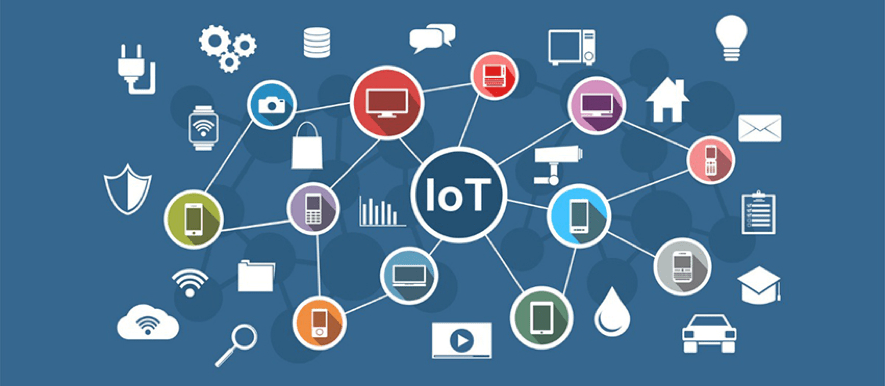
\includegraphics[width=1\textwidth]{./Figures/iot.png}
	\caption{Interconexion de dispositivos y tecnologías en IoT.}
	\label{fig:Iot}
\end{figure}

Resulta importante destacar que existe una correlación directa entre los datos y la sabiduría. Cuántos más datos se generan, más conocimiento y sabiduría pueden obtener las personas. IoT aumenta drásticamente la cantidad de datos que están disponibles para que los procesemos. Este aumento, combinado con la capacidad de Internet de comunicar estos datos, hará posible que las personas avancen aún más.En la figura \ref{fig:Sabiduria} se muestra un diagrama de la correlación entre datos y sabiduría.

\begin{figure}[ht]
	\centering
	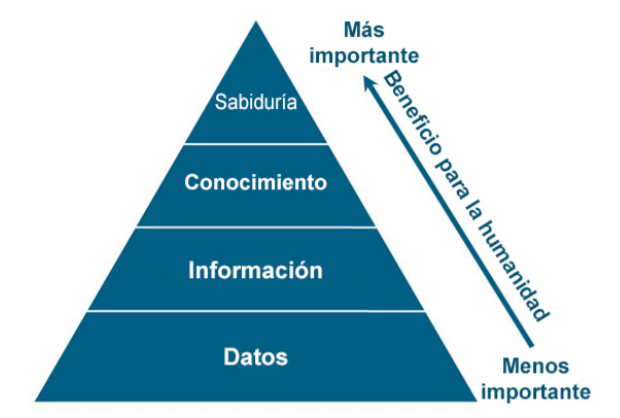
\includegraphics[width=1\textwidth]{./Figures/sabiduria.png}
	\caption{Correlación entre datos y sabiduría.}
	\label{fig:Sabiduria}
\end{figure}

Si se combina la capacidad de la próxima evolución de Internet (IoT) para percibir, recolectar, transmitir, analizar y distribuir datos a escala masiva con la manera en que las personas procesan la información, la humanidad tendrá el conocimiento y la sabiduría necesarios no solo para sobrevivir sino para mejorar y prosperar en los próximos meses, años, décadas y siglos.

En lo particular de las empresas, con IoT aparece el término de transformación digital. La misma es la aplicación de la tecnología digital para proporcionar el entorno adecuado para la innovación de las empresas y la industria. En este contexto, el desarrollo de nuestro trabajo propone realizar una transformación digital en la empresa Tenaris Metalmecánica, aprovechando estas tecnologías disruptivas.

\subsection{Control de acceso}

El control de acceso se refiere a los mecanismos que permiten o restringen la entrada de una persona o vehículo a una empresa o recinto mediante su identificación. Dentro de los principales objetivos del control de acceso incluye garantizar la seguridad y facilitar la organización empresarial. Cuando una organización instala un sistema de control de acceso, lo hace básicamente pensando en tres propósitos:
\begin{itemize}
\item Cuidar de la integridad física de las personas; es decir, evitar que ataquen a alguien.
\item Proteger la información de la compañía: bases de datos, material sensible, etc.
\item Custodiar los activos de la empresa, como los equipos electrónicos o cualquier otro bien que sea vendible.
\end{itemize}

e emplean diferentes medios para monitorear y controlar el acceso de las personas a una instalación. Décadas atrás se usaban sistemas de cerraduras y llaves; sin embargo, además de ser vulnerables, las llaves robadas o extraviadas representaban gastos adicionales para las empresas. Con el advenimiento de Internet, y principalmente de IoT el control de acceso migró a sistemas más robustos con credenciales electrónicas o identificación biométrica.

\subsubsection{Factores de autenticación}
Para un proceso de identificación, sea físico o digital, se comprueba la identidad de la persona que hace la solicitud. Esa verificación se puede ejecutar usando uno o varios factores de autenticación.

Los factores de autenticación se pueden dividir en:

\begin{itemize}
\item Lo que sé: el conocimiento que la persona tiene, puede ser un PIN, una contraseña o un patrón.
\item Lo que tengo: la identificación que posee un individuo para certificar que es él, como una credencial física o virtual.
\item Lo que soy: los rasgos corporales únicos de la persona que se utilizan para verificar la identidad (biometría).
\end{itemize}

Para aumentar el nivel de seguridad, los sistemas modernos implementan varios factores de autenticación en los puntos de acceso, combinando ``lo que tengo'' con ``lo que sé'' y con ``lo que soy'' \citep{WEBSITE:ControlAcceso}.

\subsubsection{Clasificación de sistemas de control de acceso}

Los sistemas de control de acceso para personas se clasifican por dos criterios: conexiones y método de identificación \citep{WEBSITE:ControlAccesoPersonas}.

Por su conectividad:

\begin{itemize}
\item Controles de acceso autónomos: No necesitan conectarse a la red y no guardan datos de los movimientos que se produzcan, sino que se limitan a abrir las puertas o barreras. 
\item Controles de acceso conectados en red: Estos, además de abrir accesos, registran las entradas y salidas de personas. Deben conectarse a Internet ya que la información de esos movimientos se descargará en una aplicación para poder generar informes.
\end{itemize}

Por su método de identificación:

\begin{itemize}
\item Biométricos: La identificación se produce mediante la lectura de datos físicos individuales que imposibilitan la suplantación al ser intransferibles, por lo que se consideran los más seguros. Su empleo implica el cumplimiento de la normativa en materia de protección de datos y no está permitida en todas las. Dentro de estas tenemos reconocimiento facial y huella dactilar.
\item Tarjetas: En muchas oficinas, y también en centros de trabajo como laboratorios, talleres o fábricas donde los trabajos manuales y la higiene no aconsejen utilizar la huella dactilar, se utilizan llaveros y tarjetas para identificarse en los lectores. Estas últimas son de dos clases:
	\begin{itemize}
	\item Tarjetas magnéticas: Se deben introducir en el lector por el lado de la banda magnética que contiene los datos de cada persona autorizada para abrir el acceso.
	\item Tarjetas (RFID): No requieren contacto con el lector para activar el relé que abre el acceso por radiofrecuencia, y por eso se llaman ``tarjetas de proximidad''.
	\end{itemize}
\item Contraseña numérica: algunos sistemas de control de accesos permiten fichar poniendo una contraseña en el teclado del propio terminal.
\end{itemize}

\subsubsection{Estudio de mercado}

Para nuestro trabajo se realizó un análisis de los sistemas existentes en el mercado y se encontró que la seguridad y confiabilidad de las soluciones existentes van en relación a su precio. Se detectó que la gran mayoría de los sistemas del mercado son cerrados y auto-gestionados, lo que limita su integración con otros sistemas y el valor agregado que podría darse al trabajo a implementar. Existen productos que pueden integrarse con asistentes de voz, como Echo o Alexa de Amazon o Home de Google. El problema es que a nivel empresarial la privacidad de los datos es fundamental, lo que implica que no pueden o no es deseable compartir datos con los mismos. Varios de los sistemas permiten acceso mediante huella, lo cual puede resultar muy cómodo, pero no es útil en la locación industrial donde se va a implementar el trabajo debido a que se requiere por un lado una política especial para el guardado de los datos y no divulgación de las huellas dactilares y por otro lado por el tipo de trabajo manual y falta de higiene se desaconseja. En el capítulo 4, en la sección \ref{sec:comparativa} se realiza un análisis comparativo de las soluciones estudiadas y las ventajas y desventajas de ellas contra el trabajo desarrollado. En particular se analizaron dos soluciones, una de Pronext (Pronext KY800 \citep{WEBSITE:Ponext}) y una de Samsung (Samsung SHS-H505 \citep{WEBSITE:Samsung}). Si bien dichas soluciones no son costosas y brindan algunas características interesantes como doble factor de autenticación o acceso mediante huella, no soportan conexión con sistemas externos lo cual no permite el agregado de valor a los datos, para transformarlos en información para la toma de decisiones. 


%----------------------------------------------------------------------------------------

\section{Motivación}

La empresa Tenaris Metalmecánica produce varillas de bombeo para la extracción de petróleo, para lo cual tiene una planta industrial con diferentes equipos y procesos para llevar adelante la fabricación de estos productos. Ante la necesidad continua de mejorar la calidad de los procesos de producción y los productos manufacturados a clientes, se requiere contar con alertas tempranas ante desvíos en los procesos industriales y de soporte en la empresa. Se ha detectado que existen muchos problemas recurrentes en los procesos de planta, los cuales se plantean en reuniones diarias de gestión, pero que quedan sin solución y vuelven a repetirse por no abordarlos de una manera sistemática. Muchos de estos problemas implican soluciones rápidas y automáticas y en otros casos implican generar tareas que requieren tiempo e involucramiento de diferentes actores o sectores de planta. Estos problemas han derivado a lo largo del tiempo en problemas de calidad (no conformidades), pérdida de dinero y tiempo de recursos valiosos para la empresa. 

En este sentido, se plantea la necesidad de contar con un sistema que permita detectar rápidamente los desvíos en los procesos y generar alertas tempranas o actuar automáticamente en la medida de lo posible. Existen casos donde los procesos a controlar tienen cierto grado de automatismo y se puede generar respuestas automáticas, mediante diferentes tipos de actuadores. En otros casos se generan alertas para que el personal o la gerencia tome decisiones y hay otros casos donde se deben generar tareas de control o mejoras a implementar por parte de diferentes sectores. De este modo, se logra una trazabilidad entre el problema o desvío y las acciones correctivas o preventivas a futuro. Para el caso de las tareas o flujos de trabajo manuales, el sistema debe permitir un seguimiento de las mismas y se brindar información de las tareas completas, en curso y la antigüedad de las mismas.

El sistema debe permitir la generación de alertas y la actuación desde distintos puntos, procesos y tecnologías, mediante un sistema que expone una interfaz de servicios web para su comunicación. Además, debe adaptarse a diferentes casos de uso o procesos que se irán agregando en diferentes etapas.

%----------------------------------------------------------------------------------------

\section{Objetivos y alcance}

En esta primera etapa y para el trabajo proyectado el objetivo será controlar los ingresos de terceros a la planta, para asegurar que todo tercero que acceda a planta cuenta con todos los requisitos legales y médicos al día. En caso contrario, se debe inhabilitar su acceso e informar a las áreas operativas. Se toma este caso de uso como primera prioridad, dado que cualquier accidente o problema que pueda suceder con un tercero dentro de la planta, si el mismo no contara con toda la documentación necesaria, podría incurrirse en graves problemas legales para la empresa. Durante el último año se detectaron en auditorías internas varios casos de usuarios con documentación vencida y se necesita actuar en consecuencia en lo inmediato.

El alcance de este proyecto incluye el desarrollo de una plataforma de software y módulos de actuación y sensado para el control de ingreso de terceros a planta. A su vez, la plataforma deberá quedar preparada para la incorporación futura de nuevos módulos de sensado y actuación, que deberán ser desarrollados y luego configurados pertinentemente en la plataforma, pero sin necesidades de mayores desarrollos en la misma.

Dentro de la plataforma de software se implementarán los servicios necesarios para la recepción de alarmas mediante servicios web, se generará la infraestructura y modelos de datos necesarios para modelizar alertas, tareas y actuadores genéricos. Adicionalmente, se desarrollará un módulo de sensado para leer tarjetas RFID, las cuales se asignarán a cada usuario tercero que quiera ingresar a planta y un módulo de actuación para liberar o bloquear la cerradura de entrada a la planta junta a una alarma visual que indique la habilitación o no del usuario. Ambos módulos serán componentes electrónicos o controladores que se encargarán del sensado o actuación y la comunicación de estos sensores y actuadores con la plataforma de software, bien sea mediante una red cableada o Wifi, según la disponibilidad de infraestructura del área. La plataforma de software se implementará dentro de la Intranet de la empresa, en la arquitectura existente.

No se implementarán los módulos para la configuración automática por parte del usuario de las tareas, alertas y actuadores, de modo que estas configuraciones se harán cargando datos directamente en la base de datos del sistema. Queda para una etapa posterior del proyecto desarrollar este módulo, para facilitar la configuración y agregado de nuevos módulos al sistema por parte de los usuarios, sin depender del área de sistemas. Tampoco se desarrollarán otros módulos adicionales al módulo de actuación y sensado para el control de terceros.

Para determinar si un usuario está habilitado o no a fín de ingresa a planta se consultará con un sistema de documentación de terceros que ya está operativo en la empresa. El mismo permite conocer si el tercero está activo (está prestando servicios actualmente en la empresa o fue dado de baja por fin de su contratación) y si tiene toda la documentación requerida al día. Nuestro desarrollo se comunicará con este a través de la Intranet de la empresa.

En la figura \ref{fig:Solucionbasica} se muestra el diagrama en bloques de la solución, con las interfaces del sistema: el ingreso de información desde el módulo de sensado, la interfaz de conexión entre el sistema de alertas y el sistema de documentación de terceros y las salidas del sistema al módulo de actuación, las alertas por email y las tareas generadas por el sistema a los usuarios.

\begin{figure}[ht]
	\centering
	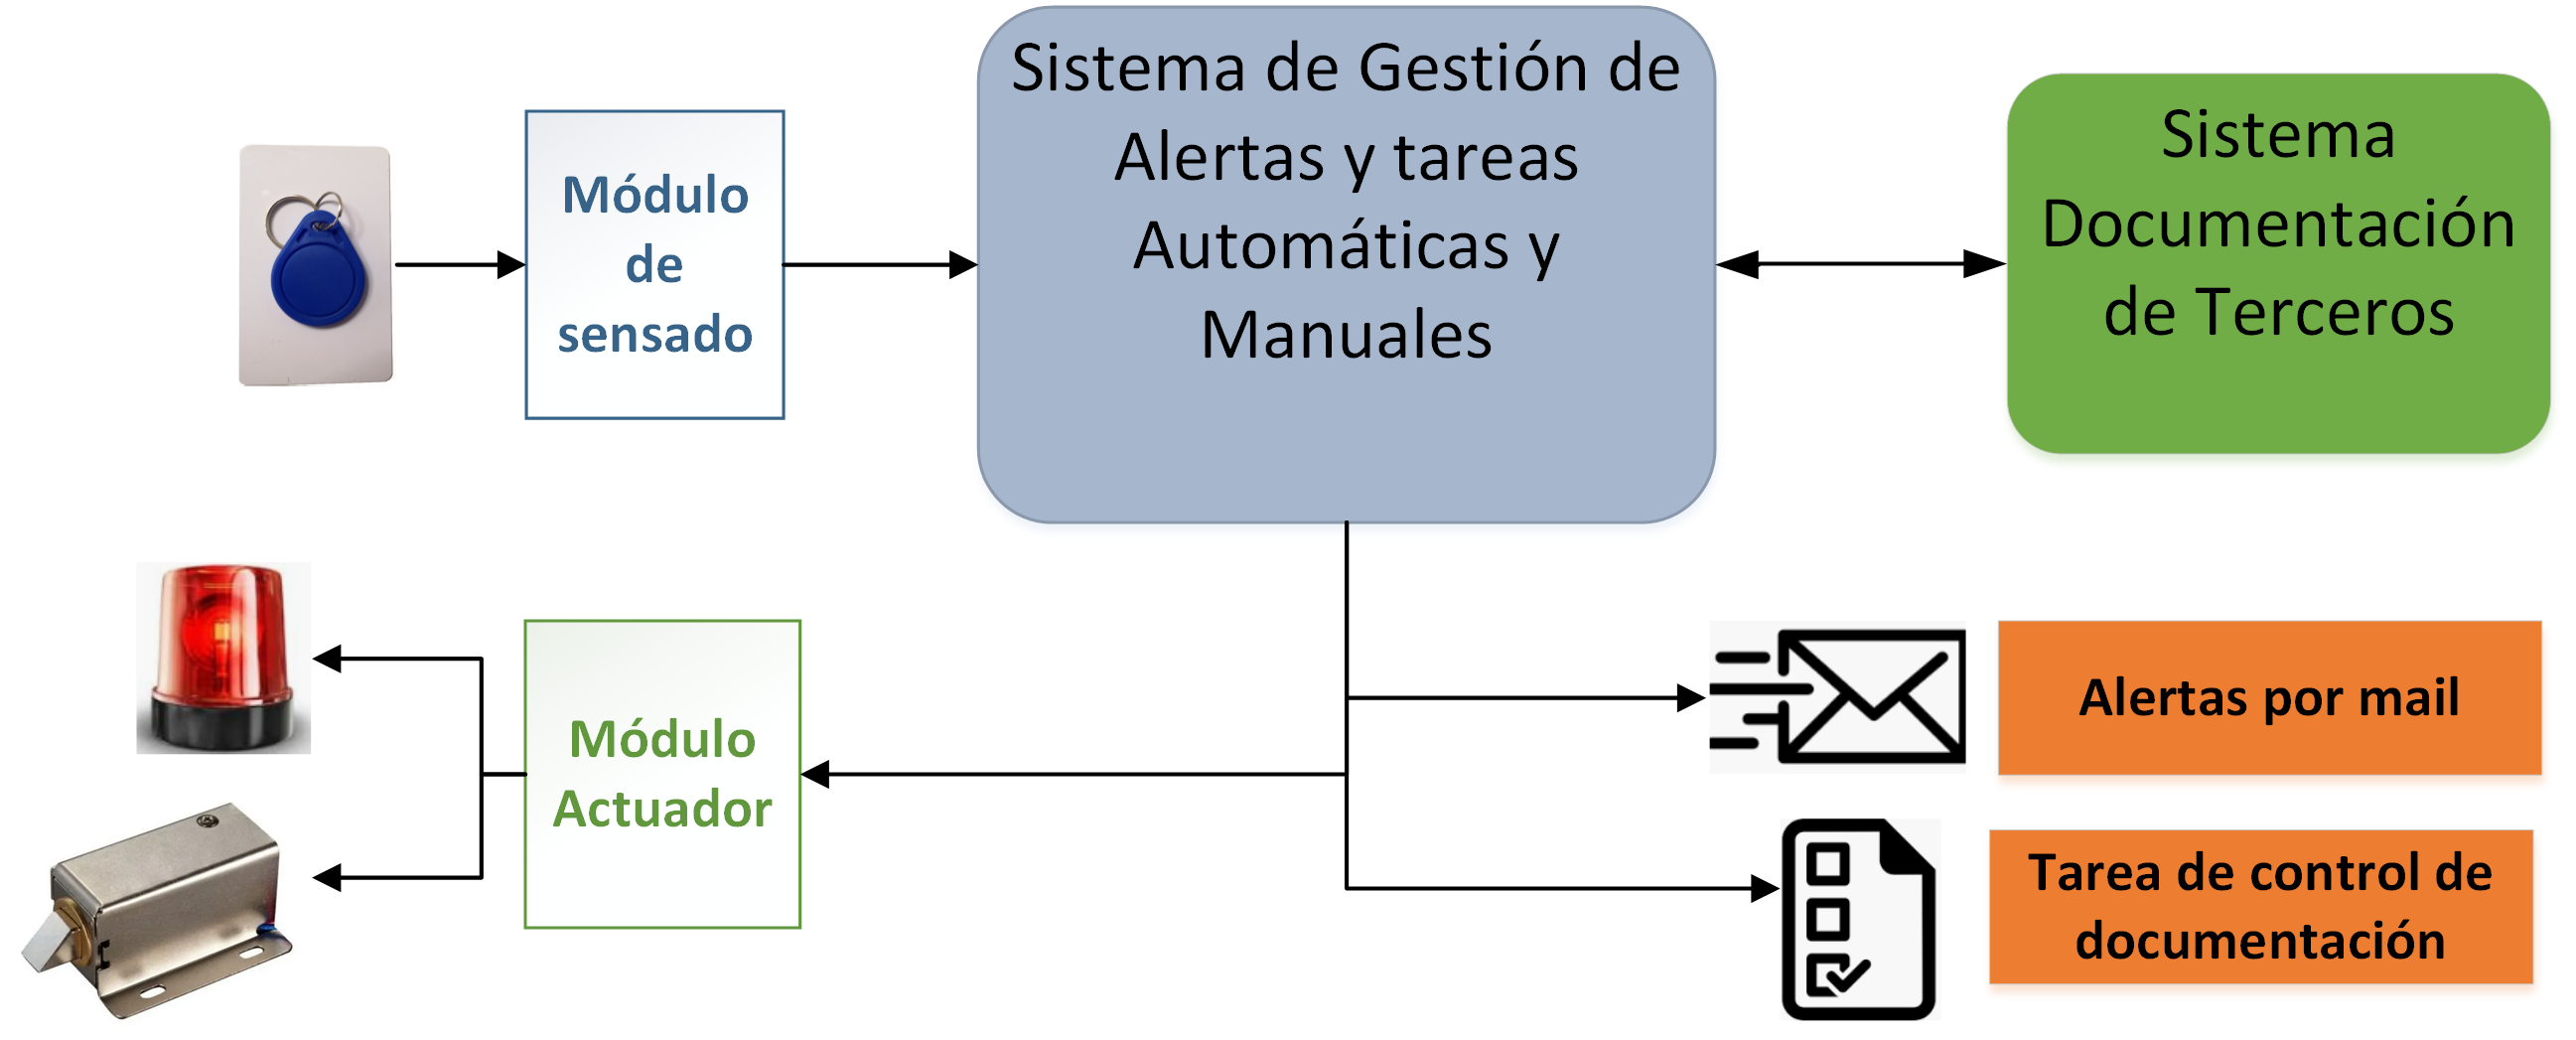
\includegraphics[width=1\textwidth]{./Figures/solucionbasica.png}
	\caption{Diagrama en bloques de la solución propuesta.}
	\label{fig:Solucionbasica}
\end{figure}




%----------------------------------------------------------------------------------------

